%	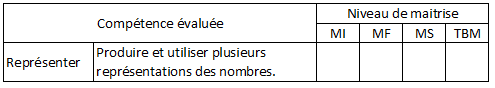
\includegraphics[scale=0.95]{competences}

\section{Divisibilité}

Pour chacun de ces nombres, dire s'ils sont divisibles par 2, 3, 5, 9 ou 10 :
\begin{questions}
	
	
	
	
	
	\question[2]  $\num{1254875}$
	\fillwithdottedlines{1.5cm}
	\begin{solution}
		
	\end{solution}
	
	\question[2]  $\num{14520}$
	\fillwithdottedlines{1.5cm}
	\begin{solution}
		
	\end{solution}

	\question[2]  $\num{2544}$
	\fillwithdottedlines{1.5cm}
	%
	\begin{solution}
	
	\end{solution}


	\question[2]  $\num{111}$
	\fillwithdottedlines{1.5cm}
	\begin{solution}
		31
	\end{solution}	 
	
\end{questions}

\newpage

\section{Simplification}

Simplifier les fractions suivantes (en détaillant)
\begin{questions}
	
	
	\question[2]  $\dfrac{33}{27}$
	\fillwithdottedlines{1.5cm}
	\begin{solution}
		
	\end{solution}

	
	
	
	
	\question[2]  $\dfrac{45}{25}$
	\fillwithdottedlines{1.5cm}
	\begin{solution}
		
	\end{solution}
	
	

	
	
	\question[2]  $\dfrac{59}{12}$
	\fillwithdottedlines{1.5cm}
	\begin{solution}
		
	\end{solution}

	\question[2]  $\dfrac{60}{45}$
	\fillwithdottedlines{1.5cm}
	\begin{solution}
		
	\end{solution}
	
	\question[2]  $\dfrac{16}{4}$
	\fillwithdottedlines{1.5cm}
	\begin{solution}
		
	\end{solution}
	
		\question[2]  $\dfrac{99}{54}$
	\fillwithdottedlines{1.5cm}
	\begin{solution}
		
	\end{solution}
	

\end{questions}


